\chapter{Anforderungen}

\section{Aufgabenstellung}
Nachfolgend ist die unterschriebene Aufgabenstellung abgebildet.

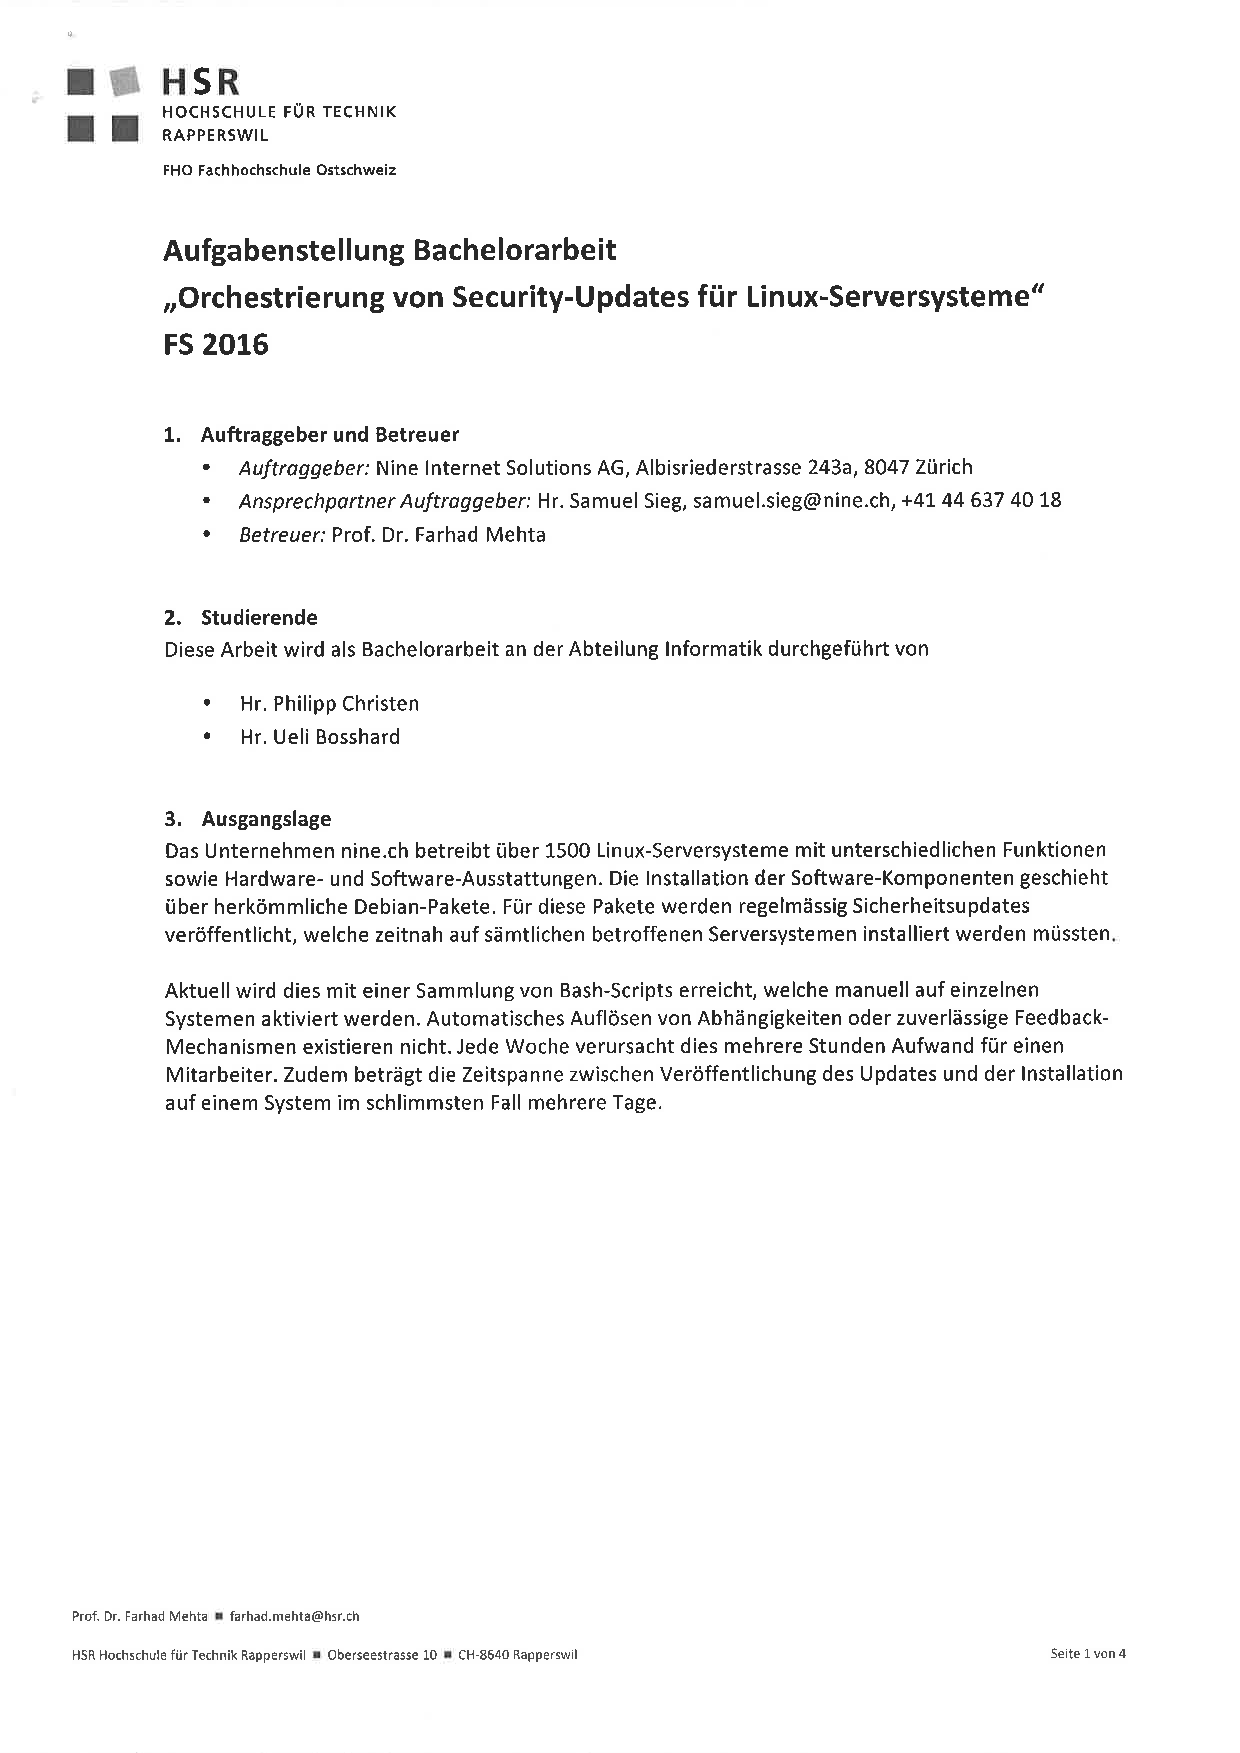
\includepdf[pages=1-,frame,scale=0.7,pagecommand={}]{files/BA_UBosshard_PChristen_SIGNED}

\section{Ausgangslage}
\xxx[Ausgangslage (Kontext) und Problembeschreibung bzw. -analyse (mit Beschreibung der
Problemtyps, also ob Fokus Lösungserstellung oder Machbarkeitsanalyse). Anforderungen spezifiziert:
Funktionale Anforderungen z.B. als Use Cases (short) oder User Stories beschrieben, alle relevanten Nichtfunktionalen Anforderungen (NFA) und Qualitätsattribute abgedeckt und überprüfbar beschrieben.]

\section{User Stories}\label{sec:pd:user-stories}

\xxx[Funktionale Anforderungen als Use Cases (short) oder User Stories
beschrieben]

\section{Nicht-funktionale Anforderungen}
%(Rahmenbedingungen, evtl. Verweis auf 1.3)

\xxx[Alle NFA/Qualitätsattribute abgedeckt und testbar beschrieben]

